\section{Summary of Paper \ref{pap:vct}}
\subsection*{"\nameref{pap:vct}"}
\subsection*{Scope and motivations}
The objective of paper \ref{pap:vct} was to propose a parametric model structure based on physical insights from CFD and FRMT inverse dynamics. The reference model from Paper \ref{pap:physics} was assumed to be close to the physically correct true model of ship manoeuvring dynamics. This model was developed with VCT (see \ref{sec:VCT}), which is based on physical first principles through CFD calculations. Paper \ref{pap:vct} investigates the identification of manoeuvring with VCT more closely, with the aim of getting even closer to the true model.

Manoeuvring models were developed for two WAPS test cases with large rudders. The models were identified by conducting VCT to obtain hydrodynamic damping coefficients and by conducting pure yaw and pure sway tests in FNPF to obtain the added masses using the Fourier series method (see \autoref{sec:fourier}). The identified force models were compared with the inverse dynamics forces of the zigzag tests to identify possible weak spots within the models.

\subsection*{Results and concluding remarks}
Propeller and rudder forces were measured during the FRMTs for Optiwise. It was found that these measured forces together with forces predicted with a hull sub module, identified from VCT data, could recreate the estimated inverse dynamics forces during zigzag maneuvers with good agreement. Much effort was therefore devoted to find a rudder force prediction model that could recreate the rudder forces for Optiwise. A modified quadratic MMG rudder model was proposed as an improved version of the original model \cite{yasukawaIntroductionMMGStandard2015}. \autoref{fig:MMG_quadratic} shows how the proposed quadratic formulation improves the fit to the VCT rudder force data.  
\begin{figure}[h]
     \centering
     \begin{subfigure}[b]{0.49\textwidth}
         \centering
         \includesvg[width=1\textwidth]{figures/results_optiwise_VCT.Y_R_MMG_original.svg}
        \caption{Original MMG rudder model.}
        \label{fig:Y_R_MMG_original}
     \end{subfigure}
     \hfill
     \begin{subfigure}[b]{0.49\textwidth}
         \centering
         \includesvg[width=1\textwidth]{figures/results_optiwise_VCT.Y_R_MMG_quadratic.svg}
        \caption{Modified quadratic MMG rudder model.}
        \label{fig:Y_R_MMG_quadratic}
     \end{subfigure}
    \caption{Rudder force during the VCT tests as a function of the effective inflow angle for the original MMG model and the modified quadratic MMG model.}
    \label{fig:MMG_quadratic}
\end{figure}

\autoref{fig:rudder_forces}  shows a comparison of rudder forces predicted with the models, measurements, and state VCT calculations which agree well. 
\begin{figure}[h]
    \centering
    \begin{subfigure}[b]{\textwidth}
        \centering
        \includesvg{figures/results_optiwise_ID.rudder_forces_zigzag 10_10.svg}
        \caption{Zigzag10/10 to port.}
        \label{fig:ID_measured_rudder_zigzag_10_10}
    \end{subfigure}
     \vfill
    \begin{subfigure}[b]{\textwidth}
        \centering
        \includesvg{figures/results_optiwise_ID.rudder_forces_zigzag 20_20.svg}
        \caption{Zigzag20/20 to starboard.}
        \label{fig:ID_measured_rudder_zigzag_20_20}
    \end{subfigure}
    \caption{Rudder forces during the zigzag tests compared to predictions with the MMG models.}
    \label{fig:rudder_forces}
\end{figure}

The total forces during the zigzag tests, including the hull and rudder predictions are shown in \autoref{fig:ID_optiwise20} which also show good agreement with the inverse dynamics forces (FRMT).

\begin{figure}[h]
    \centering
    \begin{subfigure}[b]{\textwidth}
        \centering
        \includesvg{figures/results_optiwise_ID.zigzag 10_10.svg}
        \caption{Zigzag10/10 to port.}
        \label{fig:ID_MMG_zigzag_10_10}
    \end{subfigure}
     \vfill
    \begin{subfigure}[b]{\textwidth}
        \centering
        \includesvg{figures/results_optiwise_ID.zigzag 20_20.svg}
        \caption{Zigzag20/20 to starboard.}
        \label{fig:ID_MMG_zigzag_20_20}
    \end{subfigure}
    \caption{Inverse dynamics forces during the zigzag tests compared to predictions with the MMG models.}
    \label{fig:ID_optiwise20}
\end{figure}

Closed loop simulations were also conducted as shown in \autoref{fig:sim_optiwise} with very good agreement for the zigzag20/20 tests and a bit less agreement for the zigzag10/10 tests.
For Optiwise it can therefore be concluded that
the VCT data contained correct damping forces during the maneuvers, which were well
described by the chosen model structure including the proposed rudder model, and also that the method used to determine added masses gave reasonable values.
\begin{figure}[h]
     \centering
     \begin{subfigure}[b]{0.49\textwidth}
         \centering
         \includesvg{figures/results_optiwise_ID.closed loop zigzag 10_10 port.svg}
         %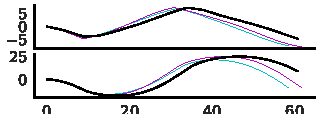
\includegraphics[]{figures/results_optiwise_ID.closed loop zigzag 10_10 port.pdf}
        \caption{Zigzag10/10 to port.}
        \label{fig:sim_optiwise_10_port}
     \end{subfigure}
     \hfill
     \begin{subfigure}[b]{0.49\textwidth}
         \includesvg{figures/results_optiwise_ID.closed loop zigzag 10_10 stbd.svg}
         %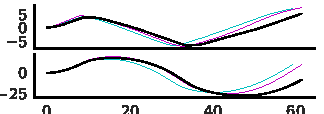
\includegraphics[]{figures/results_optiwise_ID.closed loop zigzag 10_10 stbd.pdf}
        \caption{Zigzag10/10 to starboard.}
        \label{fig:sim_optiwise_10_stbd}
     \end{subfigure}
     \vfill
     \begin{subfigure}[b]{0.49\textwidth}
         \centering
         \includesvg{figures/results_optiwise_ID.closed loop zigzag 20_20 port.svg}
         %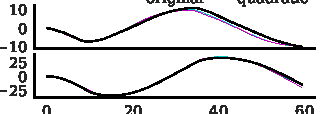
\includegraphics[]{figures/results_optiwise_ID.closed loop zigzag 20_20 port.pdf}
        \caption{Zigzag20/20 to port.}
        \label{fig:sim_optiwise_20_port}
     \end{subfigure}
     \hfill
     \begin{subfigure}[b]{0.49\textwidth}
         \includesvg{figures/results_optiwise_ID.closed loop zigzag 20_20 stbd.svg}
         %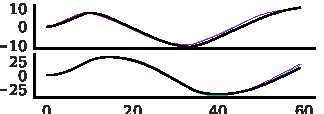
\includegraphics[]{figures/results_optiwise_ID.closed loop zigzag 20_20 stbd.pdf}
        \caption{Zigzag20/20 to starboard.}
        \label{fig:sim_optiwise_20_stbd}
     \end{subfigure}
     
        \caption{Comparison of zigzag tests between Optiwise experiments (black) and simulations with the MMG original (cyan) and MMG quadratic (purple).}
        \label{fig:sim_optiwise}
\end{figure}